\title{CS 513 Assignment 4}
\author{Ruochen Lin}
\documentclass[11pt]{article}
\usepackage{amsmath,amsfonts,amssymb,amsthm}
\usepackage{mathtools}
\usepackage{commath}
\usepackage{setspace}
\usepackage{algorithm,algorithmic}
% \setmonofont{hack}
\begin{document}
\maketitle
\section{}
\subsection{}
In the $k+1$th step of Gaussian elimination for a $m\times m$ square matrix, the first $k$ columns and rows are untouched; thus we are effectively performing the step on a $(n-k)\times(n-k)$ square matrix. If we call this square matrix $B$, and the resulting $(n-k-1)\times(n-k-1)$ matrix $C$, then the entries of $C$ is given by the following equation:
\begin{equation}\begin{split} 
C_{i,j}&=B_{i+1,j+1}-\frac{B_{i+1,1}}{B_{1,1}}B_{1,j+1}\\
\Leftrightarrow C_{j,i} &= B_{j+1,i+1} - \frac{B_{j+1,1}}{B_{1,1}}B_{1,i+1}.
\end{split}\nonumber\end{equation} 
If $B$ is symmetric, then we have $B_{i+1,j+1} = B_{j+1,i+1}$, $B_{i+1,1} = B_{1,i+1}$, and $B_{1,j+1} = B_{j+1,1}$, which leads to $C_{i,j} = C_{j,i}$. In other words, if we start with a symmetric matrix at the beginning of the step, then the resulting matrix will also be symmetric. Note that we do start with a symmetric matrix, $A$; thus the lower right sqaure matrices after each step of Gaussian elimination will all be symmetric.

\subsection{}
We can modify the algorithm of the LU-factorization for symmetric matrices, utilizing the theorem in the preceeding part: in the $k$th step of the Gaussian elimination, we can only update the entries in the upper triangular part of the remaining $(m-k-1)\times(m-k-1)$ block at bottom right. The pseudocode of such algorithm is the following:
\begin{algorithm}[H]
\caption{LU-factorization for a symmetric matrix A}
\begin{algorithmic}
	\STATE L = eye(m)
	\STATE U = A
    \FOR{i = 1 : m - 1}
		\FOR{j = i + 1 : m}
			\STATE L(j,i) = U(i,j) / U(i,i)
			\STATE U(j,i) = 0
			\FOR {k = j : m}
				\STATE U(j,k) = U(j,k) - L(j,i) * U(i,k)
			\ENDFOR
		\ENDFOR
    \ENDFOR
\end{algorithmic}
\end{algorithm}

\subsection{}
It's easy to see that the most executed part of the algorithm is the inner most loop with the dummy index $k$. In lieu of the analysis in class, if we only count multiplications, then each execution of the inner most loop contributes exactly $1$ operation. The total number of multiplications, $N(m)$, can be estimated as the following:
\begin{equation}\begin{split} 
N(m) &= \sum_{i=1}^{m-1} \sum_{j=i+1}^m \sum_{k=j}^m 1\\
&= \sum_{i=1}^{m-1} \sum_{j=i+1}^m (m - j + 1) \\
&= \sum_{i=1}^{m-1} \Big[ 1 + 2 + \cdots + (m-i) \Big] \\
&= \sum_{i=1}^{m-1} \frac{(m-i)(m-i+1)}2 \\
&= \sum_{i=1}^{m-1} \Big[ \frac{(m-i)^2}2 + O(m) \Big]\\
&= \frac12\Big[ 1^2 + 2^2 + \cdots + (m-1)^2 \Big] + O(m^2) \\
&= \frac12\cdot \frac{(m-1)m(2m-1)}6 + O(m^2)\\
&=\frac{m^3}6 + O(m^2).
\end{split}\nonumber\end{equation} 
Thus, our current algorithm is almost twice as fast as ordinary Gaussian elimination.

\subsection{}
To verify our analysis in the preceeding part, we have created random symmetric matrices with dimensions ranging from 10 to 100, and see how much time is needed by the two algorithms to LU-factorize the matrix. At each dimension, the time reading is averaged over 100 runs. From Fig 1, we can see that the original algorithm does take around twice of the time required by our algorithm, corroborating our analysis. In addition, the $O(m^3)$ cost can be qualitatively verified from the fact that, when the dimension is doubled, say from 50 to 100, the time elapsed in the two algorithms increaded by factors of 7.13 and 6.25 in the two alforithms, respectively, which are close to $2^3 = 8$.
\begin{figure}[t]
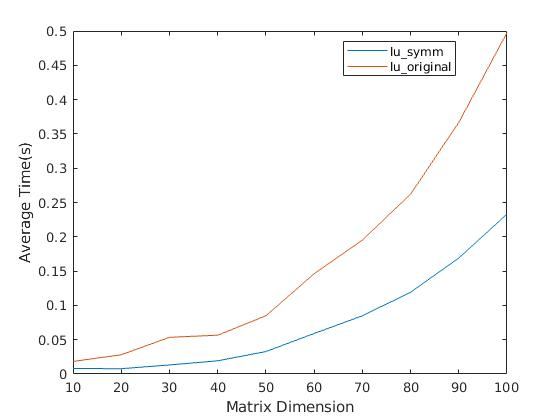
\includegraphics[width=8cm]{matlab/prob1d.jpg}
\centering
\caption{Plot of the time needed by LU-factorization considering symmetry and the original LU-factorization algorithms to decompose random symmetric matrices.}
\end{figure} 
\end{document}
